\documentclass[tikz,border=10pt]{standalone}
\usepackage{tikz}
\usetikzlibrary{positioning, arrows.meta, shapes.geometric, fit, backgrounds, calc}

\begin{document}
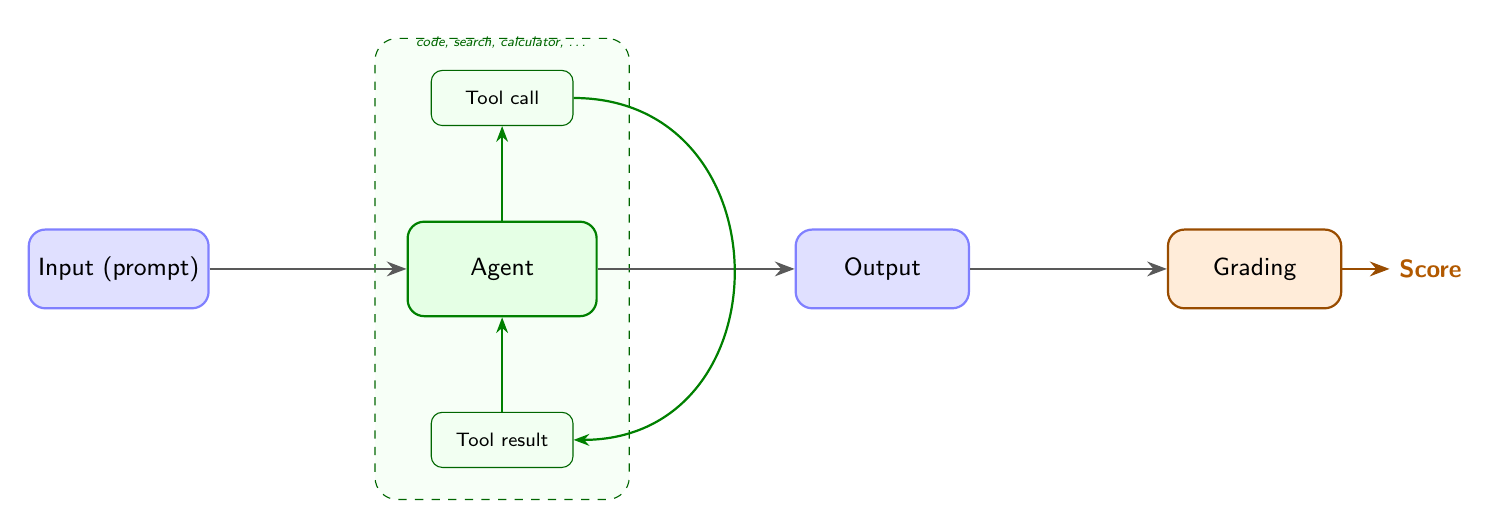
\begin{tikzpicture}[
    node distance=1.8cm and 2.2cm,
    box/.style={rectangle, draw, rounded corners=6pt, minimum width=2.2cm, minimum height=1cm, thick, font=\sffamily\small},
    input/.style={box, fill=blue!12, draw=blue!50},
    agent/.style={box, fill=green!10, draw=green!50!black, minimum width=2.4cm, minimum height=1.2cm},
    output/.style={box, fill=blue!12, draw=blue!50},
    grading/.style={box, fill=orange!15, draw=orange!60!black},
    toolbox/.style={rectangle, draw, rounded corners=4pt, fill=green!5, draw=green!40!black, minimum width=1.8cm, minimum height=0.7cm, font=\sffamily\scriptsize},
    arrow/.style={-{Stealth[length=2.5mm]}, thick, gray!70!black},
    looparrow/.style={-{Stealth[length=2mm]}, thick, green!50!black},
]

% Main flow nodes
\node[input] (input) {Input (prompt)};
\node[agent, right=2.5cm of input] (agent) {Agent};
\node[output, right=2.5cm of agent] (output) {Output};
\node[grading, right=2.5cm of output] (grading) {Grading};

% Tool use loop
\node[toolbox, above=1.2cm of agent] (toolcall) {Tool call};
\node[toolbox, below=1.2cm of agent] (toolresult) {Tool result};

% Main flow arrows
\draw[arrow] (input) -- (agent);
\draw[arrow] (agent) -- (output);
\draw[arrow] (output) -- (grading);

% Tool use loop arrows
\draw[looparrow] (agent.north) -- (toolcall.south);
\draw[looparrow] (toolcall.east) to[out=0, in=0, looseness=1.6] (toolresult.east);
\draw[looparrow] (toolresult.north) -- (agent.south);

% Score output
\node[right=0.6cm of grading, font=\sffamily\small\bfseries, color=orange!70!black] (score) {Score};
\draw[arrow, orange!60!black] (grading) -- (score);

% Labels
\node[above=0.15cm of toolcall, font=\sffamily\tiny\itshape, color=green!40!black] {code, search, calculator, \ldots};

% Dashed box around agent + tools
\begin{scope}[on background layer]
    \node[draw=green!40!black, dashed, rounded corners=8pt, fit=(toolcall)(agent)(toolresult), inner sep=0.4cm, fill=green!3] {};
\end{scope}

\end{tikzpicture}
\end{document}
